\documentclass[11pt]{article}
\usepackage[includeheadfoot, top=1.0in, bottom=1.0in, hmargin=1.0in]{geometry}
\usepackage[utf8]{inputenc}
\usepackage{fancyhdr}
\pagestyle{fancy}
\usepackage{setspace}
\usepackage{tabularx}
\usepackage{xcolor}
\usepackage{cancel}
\usepackage{amsmath,amsfonts}
\usepackage{graphicx}
\usepackage{siunitx}
\usepackage{amssymb}

\usepackage[hyphens]{url}
\usepackage{hyperref}

\lhead{Astronomy Lab II}
\rhead{Fall 2024}
\lfoot{Porter}
\rfoot{Wed 6-9pm}
\cfoot{\thepage}

\begin{document}

\begin{center}
\huge{Lab 2: Exploring the Multiwavelength Universe: The Electromagnetic Spectrum and Intro to Telescopes}\\ \medskip \Large{September 18, 2024}
\end{center}

\medskip \noindent
\textbf{Please show all work and circle/highlight your final answers.}

%%%%%%%%%%%%%%%%%%%%%%% INTRO %%%%%%%%%%%%%%%%%%%%%%%
\section{Introduction: Let There Be Light}
At its core, observational astronomy is the art of collecting light. All luminous matter in the Universe -- from the tiniest grain of dust to the most massive cluster of galaxies -- emits light in some shape or form. As astronomers, it's our job to capture and interpret this ever-present light.

\medskip \noindent
While some light can be effectively processed by the naked eye (we call this ``visible'' or ``optical'' light), the majority of light in the Universe is imperceptible to humans. Electromagnetic radiation (just a fancy, science-y term for light) spans a broad \emph{spectrum} of flavors, from low-frequency radio waves to high-energy gamma rays (see Figure \ref{fig:spectrum}). Astronomical objects emit electromagnetic radiation across the entire spectrum; therefore, in order to fully understand the Universe, we must be able to observe all varieties of light. While we as humans cannot \emph{see} microwaves or radio waves or X-rays, we are more than capable of building special detectors that can. Collectively, we refer to these detectors as ``telescopes.''

\medskip \noindent
In this lab, you will learn about the variety of light comprising the ``electromagnetic spectrum.'' You will explore a range of astronomical objects producing light in all regions of the spectrum, thus demonstrating the need for a wide array of specialized telescopes. After completing this lab, you should have a deeper understanding of the nature of light, of what it means to ``observe'' the Universe, and of the utility of telescopes. These concepts form the foundations of modern astronomy. 

%%%%%%%%%%%%%%%%%%%%%%% LIGHT %%%%%%%%%%%%%%%%%%%%%%%
\section{The Anatomy of a Light Wave}
Light can be thought of as either a \emph{wave} (often referred to as an ``electromagnetic'' wave) or as a \emph{particle} (called a ``photon''). While both descriptions of light are perfectly valid, as light is both a particle and a wave, we'll primarily be focusing on the wave nature of light in this lab. When physicists refer to ``waves,'' they're referring to steady, propagating wiggles (or, in technical terms, ``oscillations''), like those illustrated in Figure \ref{fig:lightwaves} and in the slinky demonstration. These waves are comprised of a series of alternating \emph{peaks} (high points) and \emph{troughs} (low points); we can therefore characterize a wave by measuring its \emph{amplitude} (half the vertical distance from the bottom of a trough to the top of a peak) and its \textbf{\emph{wavelength}} (the horizontal distance from peak to peak or from trough to trough). For a light wave, the amplitude tells us how bright (or \emph{intense}) the light is. The relative occurences or "speed" of a wave, characterized by the number of waves per second ($s^{-1}$, also known as "Hertz") are called \textbf{\emph{frequency.}} Meanwhile, the wavelength controls the ``identity'' of a light wave -- the wavelength dictates what color the light will be, how much energy is carried by the light, how deeply the light can penetrate into matter, and more. The wavelength is the key property that we'll be exploring in today's lab. Wavelength ($\lambda$) and frequency ($\nu$) can be related to the speed of light ($c$) by:

\begin{equation}
    c = \lambda \nu
\end{equation}

where $\nu$ is in units of $s^{-1}$, and wavelength has the same units as the distance in $c$. For example, if $c$ is given in $m \; s^{-1}$, $\lambda$ will have units of meters. 

\medskip \noindent
Figure \ref{fig:lightwaves} shows only the wavelength range of ``visible'' light -- the light that we, as humans, can see with our naked eyes. Importantly, however, light can exist at wavelengths far longer and far shorter than the visible range, filling out the entire \emph{\textbf{electromagnetic (EM) spectrum}} (Figure \ref{fig:spectrum}). At the longest wavelengths, we have \emph{radio waves}; as we decrease the wavelength, we move through \emph{microwaves}, \emph{infrared light}, \emph{visible light}, \emph{ultraviolet light}, \emph{X-rays}, and \emph{gamma rays}. The wide variety of light that shines throughout the Universe makes observational astronomy an extremely rich field of study. 

\begin{figure}[t!]
    \centering
    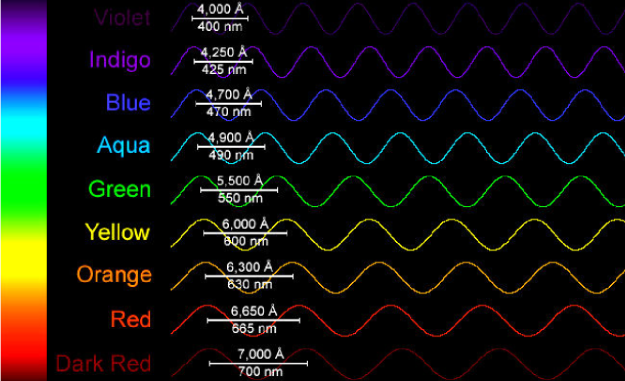
\includegraphics[width=0.8\textwidth]{Figures/optical.png}
    \caption{A collection of light waves with varying \emph{wavelengths}. The wavelengths are reported both in units of nanometers (nm, $10^{-9}$ meters) and in units of angstroms (\AA, $10^{-10}$ meters).}
    \label{fig:lightwaves}
\end{figure}

\begin{figure}
    \centering
    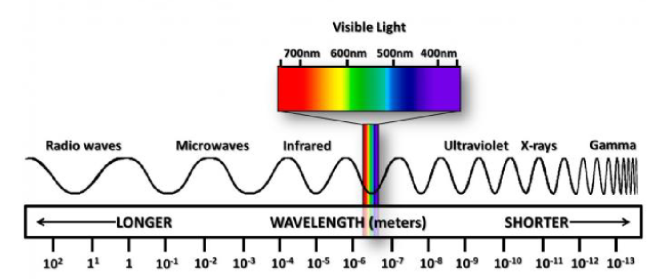
\includegraphics[width=0.8\textwidth]{Figures/emspectrum.png}
    \caption{The electromagnetic spectrum: the broad assortment of light that permeates the Universe.}
    \label{fig:spectrum}
\end{figure}
\medskip
\noindent
Let's think a little deeper about the electromagnetic spectrum. \textbf{Record your responses in your lab write-up}.
\begin{enumerate}
    \item Note the huge range of wavelengths covered by the electromagnetic spectrum (Figure \ref{fig:spectrum}). By how many orders of magnitude is the wavelength of a long radio wave (around $10^2$ m) greater than the wavelength of a gamma ray (around $10^{-13}$ m)? \textbf{You do not need complete sentences for this question, but show your work.}

    \item From the slinky demonstration, Figure \ref{fig:lightwaves}, and the formula given, what happens to the \emph{frequency} of the wave as the \emph{wavelength} increases? 
    
    \item The electromagnetic spectrum is not just relevant in astronomy -- we experience almost all wavelengths of the spectrum in our daily lives. For each region of the EM spectrum (radio, microwave, infrared (IR), visible, ultraviolet (UV), X-ray, gamma), list one or two sources of that type of light that we may find on Earth. \textbf{You do not need complete sentences for this question; a list is fine.} (\textit{Hint}: this website has some fun examples: \url{https://imagine.gsfc.nasa.gov/science/toolbox/emspectrum1.html})
    
    \item The average human body cell is 100 $\mu m$ in diameter. Compare this to the typical wavelength of a radio wave and to the typical wavelength of a gamma ray. Why do you think gamma rays are harmful to humans but radio waves are not?
    
    \item Navigate to \url{https://javalab.org/en/electromagnetic_waves_en/}. In the applet window, you can click and drag the mouse up and down to explore different regions of the electromagnetic spectrum.
    \begin{enumerate}
        \item As you drag the burgundy arrow from the top of the spectrum (the radio range) to the bottom of the spectrum (the X-ray range), describe qualitatively what happens to the propagating wave.
        
        \item When the burgundy arrow is near the top of the spectrum, the wave appears stationary and flat. Why is this the case?
    \end{enumerate}
    
    \item Different wavelengths of light have different \emph{optical properties}, meaning that they behave differently when sent through a prism or lens or when bounced off a mirror. This fact forms the basis of the extremely important technique of \textbf{\emph{spectroscopy}}, which we will explore at length in the next lab. For now, navigate to \url{https://javalab.org/en/electromagnetic_waves_around_of_visible_rays_en/}. In the applet window, you can click and drag the mouse up and down to vary the wavelength of light passing through the prism.
    \begin{enumerate}
        \item Light is ``bent'' as it travels through a prism. As you vary the wavelength from long wavelengths to short wavelengths, how does the degree of bending vary? Are shorter wavelengths bent more than longer wavelengths, or vice versa?
        
        \item This simulation only shows a \emph{single} wavelength of light passing through the prism at any given time. If we instead sent ``white light'' (an equal mixture of all wavelengths) through the prism, what do you expect the light pattern emerging from the prism to look like? 
        
        \item If we were instead to shine \emph{starlight} through the prism, what could the resulting light pattern tell us about the star? (give your best guess -- we'll look at this in more detail next week. I'm not expecting a correct answer here!)
        
    \end{enumerate}
\end{enumerate}

%%%%%%%%%%%%%%%%%%%%%%% MULTIWAVELENGTH UNIVERSE %%%%%%%%%%%%%%%%%%%%%%%
\section{The Multiwavelength Universe}
The night sky shines in all wavelengths of the electromagnetic spectrum. All ordinary matter -- including that which makes up tiny dust grains, planets, stars, galaxies, etc. -- interacts with or produces light, filling the Universe with a whole zoo of different light waves. In these next few sections, we'll explore our ``Multiwavelength Universe'' in a little more depth.

\medskip \noindent
First, go to this website: \url{https://www.nao.ac.jp/study/multiwave/en/}; we'll be using this site for the next few sections of this lab. Once the site loads, click the ``start'' button in the middle of the screen. The landing page shows the electromagnetic spectrum at the bottom of the screen, with each region labeled. Clicking on any of these labels will show you an image of the Antennae Galaxies composed of light from that particular region of the spectrum (with the exception of gamma rays, for which an image of the Antennae Galaxies is not shown). Moreover, once you've clicked on a specific wavelength range, you can scroll up or down (or use the dots on the right side of the screen) to learn more about the astronomical objects and phenomena that emit this light.

\begin{enumerate}
    %\setcounter{enumi}{6}
    \item You and a partner will be assigned a region of the electromagnetic spectrum.  For your region, add 1-2 slides to this deck \url{https://docs.google.com/presentation/d/1fOSiy4spX8OfYxKFJ6j_qUAxhfuC_hzmMonFpjghqtY/edit?usp=sharing} that briefly describes:
    \begin{itemize}
        \item what we can learn about the Antennae Galaxies by observing in this wavelength range
        \item two astrophysical phenomena that emit this type of light (\textit{Hint: }Click on ``Wavelength Guide" on the bottom of the page, and navigate to ``Wavelengths and Targets". Click on the objects in your wavelength range to learn more about them.)
        \item what telescopes we can use to observe in this range (\textit{Hint: }Navigate to ``Wavelengths and Telescopes". Click on the telescopes in your wavelength range to learn more about them.)
    \end{itemize} 
    \item With your partner, prepare a ~1-2 minute presentation to give to the class. \textbf{No need to include the slide or presentation in your write-up}; I will grade from the document itself. You will get the points for this part as long as your name is on a slide, your slide contains the requested information, and you participated in the creation and presentation.
    \item As you listen to other groups' presentations, record in your lab write-up what you can learn from \textbf{each} region of the electromagnetic spectrum, and which telescopes are used to observe in \textbf{each} region. \textbf{You do not need complete sentences for this question, a list is fine.}
\end{enumerate}

%%%%%%%%%%%%%%%%%%%%%%% TELESCOPES %%%%%%%%%%%%%%%%%%%%%%%
\section{Why do we need so many telescopes?}
Using what you learned from your classmates' presentations, \textbf{answer the following questions in your lab write-up}.  (If you need a reminder, you can find this information by navigating to the ``Wavelength Guide'' and using the ``Wavelengths and Telescopes'' and ``Wavelengths and Targets'' tab, located at the bottom of the screen).
\begin{enumerate}
    %\setcounter{enumi}{7}
    \item A few years ago, the brand new \textbf{James Webb Space Telescope} (JWST) was launched into space. Many news outlets have stated that JWST will ``replace'' the Hubble Space Telescope. Explain why this statement is not fully accurate. What telescope would it make more sense to label as the ``predecessor'' to JWST? Take a quick look at this JWST fact sheet: \url{https://jwst.nasa.gov/content/webbLaunch/assets/documents/WebbFactSheet.pdf}. Briefly describe two science cases that JWST will be (or has been) focusing on.
    
    \item The Atacama Large Millimeter/submillimeter Array -- or \emph{ALMA} -- is an array of telescopes in Chile that has been revolutionary for the study of planet formation and the study of black hole structure. List one type of astronomical object that ALMA can see well and very briefly describe this object. Recently, the field of ``submillimeter'' astronomy has received increased attention for its ability to probe star formation and cosmology -- why do you think this field is called ``submillimeter'' astronomy? 
    
\end{enumerate}

%%%%%%%%%%%%%%%%%%%%%%% ATMOSPHERE %%%%%%%%%%%%%%%%%%%%%%%
\section{The Earth's atmosphere: Astronomy's greatest enemy}

Light propagates perfectly fine through vacuum (the complete absence of matter), but as soon as we introduce matter -- like the gas in the Earth's atmosphere -- we run into trouble. As light passes through our atmosphere, turbulent gas scatters and deflects this light, affecting the clarity of ground-based telescope observations (in astronomy jargon, we say that the atmosphere affects the \emph{``seeing''} of our telescopes). Moreover, certain molecules in our atmosphere -- like water, carbon dioxide, and ozone -- can \emph{absorb} incoming light, completely preventing some wavelengths from reaching the ground. So, while the Earth's atmosphere is fantastic for life on Earth, it's disastrous for ground-based astronomy.

\medskip \noindent
Let's explore the effects of the Earth's atmosphere in a bit more depth. First, navigate back to \url{https://www.nao.ac.jp/study/multiwave/en/}. Go back to the ``Wavelength Guide'' page (located at the bottom of the screen), and now click on the ``Wavelength and Atmospheric Penetration'' tab. This page should display a graphic illustrating how far different wavelengths of light can travel through our atmosphere. Using this diagram, answer the following questions. \textbf{Record your responses in your lab write-up}.
\begin{enumerate}
    %\setcounter{enumi}{12}
    \item In which wavelength ranges can light reach the surface of the Earth (i.e., an altitude of 0 km)? Referring back to the ``Wavelengths and Telescopes'' tab, what are some \emph{ground-based} telescopes that observe in these wavelength ranges? Where are these telescopes located? (\textit{Hint}: you can click on the telescope name to find the location) \textbf{This answer doesn't need complete sentences; it can be a list.}
    
    \item Which wavelengths are affected the most by the atmosphere? Referring back to the ``Wavelengths and Telescopes'' tab, what are some telescopes that observe at these wavelengths? Where are these telescopes located? \textbf{This answer doesn't need complete sentences; it can be a list.}
    
    \item Many ground-based telescopes, like the Subaru Telescope and the Keck Observatory, are built on the summits of very tall mountains. Why is the top of a mountain an optimal location for a telescope? (\textit{Hint}: think about the air quality on top of a mountain vs. the air quality at lower altitudes)
    
    \item Many ground-based telescopes, like ALMA and ACT, are built within extremely dry deserts. Why is a desert an optimal location for a telescope? (\textit{Hint}: think about the air quality in a desert vs. the air quality in a moister environment)
    
    \item What are some benefits of space-based telescopes, like Hubble and James Webb? What might be some drawbacks?
\end{enumerate}

%%%%%%%%%%%%%%%%%%%%%%% SATELLITES and LAND ISSUES %%%%%%%%%%%%%%%%%%%%%%%
\newpage
\section{Current Problems with/for Telescopes}
\subsection{Satellites: Sometimes technology is the enemy!}

If you've ever looked up at the night sky to see a blinking light slowly moving across the sky, chances are that you've seen a satellite! Even though they orbit the planet at relatively low heights, satellites are rather bright (looking very similar to stars to us on Earth). Furthermore, as they become more affordable to build and launch with private companies like SpaceX, the population of satellites used for purposes such as GPS, national defense, weather, and more recently, Internet services (Starlink, for example), they've begun to pose a new problem to astronomers. See Figure \ref{fig:satellites} for an example.

\begin{figure}
    \centering
    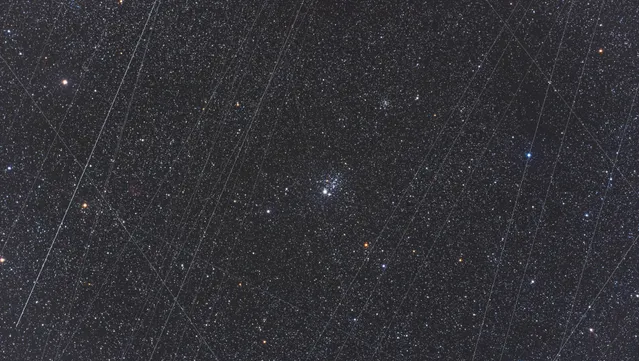
\includegraphics[width=0.5\linewidth]{Figures/satellites.png}
    \caption{Star cluster NGC 456 from the constellation Cassopeia. The streaks of light show satellite paths over the image after only 36 minutes of exposure time. Credit: Alan Dyer/VW Pics/Universal Images Group via Getty Images.}
    \label{fig:satellites}
\end{figure}

\medskip \noindent
Spend a few minutes investigating some sources on how satellites impact astronomers. Some good examples are \url{https://www.space.com/satellite-megaconstellations-spacex-starlink-interference-astronomy}, \url{https://earthsky.org/space/how-satellites-harm-astronomy-whats-being-done/}, or \url{https://www.scientificamerican.com/article/satellite-constellations-are-an-existential-threat-for-astronomy/}. Using what you've found, answer the following question. \textbf{Record your responses in your lab write-up}.
\begin{enumerate} 
    \item What are the drawbacks of increased satellite usage on astronomy? Give an example of something being done to navigate this problem. Include your source.
\end{enumerate}

\subsection{Land Conflict: Where do telescopes go?}

While astronomers usually devote most of their time to securing funding, resources, conducting science, and trying to advocate for telescopes to be built, we also have a responsibility to be good citizens and understand how our science can affect ethics.

One of the biggest examples of ethics in astronomy is the construction of large ground-based telescopes in Hawai'i, specifically on the mountain (and dormant volcano) of Mauna Kea. Many telescopes are based in Hawai'i because the atmospheric conditions and elevation (like you just reviewed in Section 5) are the most ideal on the planet, and the area is more habitable for humans and construction than mountains such as the Andes. Can you imagine being an astronomer and observing on a cold, snowy mountain where few people live? This location in Hawai'i has no significant competitors for astronomers, making it one-of-a-kind. 

However, native Hawai'ians have opposed the construction of such telescopes: the mountain is incredibly sacred to Hawai'ian culture, literally representing the home of the gods and center of the universe. Hundreds of native Hawai'ians have protested the further construction of telescopes on their sacred land, feeling as if they have lost the rights to their ancestral lands.

Think about both sides of the conflict; please feel free to research additional sources if you need to. This question is asking for your opinion on the issue and there is no correct answer. Please be \emph{mindful} and \emph{respectful} of all peoples and cultures in your answer. \textbf{Record your answer in your lab write-up.}

\begin{enumerate} 
    \item Do you think astronomers should be permitted to build additional telescopes in Hawai'i? How do you think astronomers should approach ethical problems like the one above? 
    
    If you aren't sure on your stance to the above questions, are there any current approaches that you agree/disagree with, and why?
\end{enumerate}

%%%%%%%%%%%%%%%%%%%%%%% CONCLUSIONS %%%%%%%%%%%%%%%%%%%%%%%
\section{Wrapping things up}

Complete this section by yourself. These questions are graded for \emph{completion} (quality of writing), but you should still be putting effort into your answers. My goal is to ensure that everyone leaves the lab understanding the main ideas, and if not, what I need to go over. \textbf{Record your responses in your lab write-up}. 
\begin{enumerate}
    
    \item Provide a qualitative description of the electromagnetic spectrum. How does the wavelength of light tie into the electromagnetic spectrum?
    
    \item Briefly explain the importance of observing the Universe in multiple wavelengths. 
    
    \item Why do we need so many different telescopes? Why do we need both space telescopes and ground telescopes?

\end{enumerate}

\end{document}
